% \begin{figure}[htbp]
% \centering
% \begin{tikzpicture}[scale=1.0, every node/.style={align=center}]
%   % Circle centers
%   \coordinate (A) at (0,0);
%   \coordinate (B) at (2.2,0);
%   \coordinate (C) at (1.1,1.8);

%   % Circles (grayscale, subtle)
%   \draw[thick] (A) circle (2cm);
%   \draw[thick] (B) circle (2cm);
%   \draw[thick] (C) circle (2cm);

%   % Set labels
%   \node[above left=0.1cm of A] {\textbf{A: Conceptual theory}};
%   \node[above right=0.1cm of B] {\textbf{B: Methods \& measurement}};
%   \node[above=0.1cm of C] {\textbf{C: Managerial practice \& design}};

%   % Intersection labels (placed by eye; adjust if needed)
%   % A ∩ B
%   \node[text width=4.1cm] at (1.1,-0.4) {\textbf{A ∩ B}\\Operational foundations of resilience\\(behavioral \& computational indicators; ABM)};
%   % A ∩ C
%   \node[text width=4.1cm] at (0.2,1.0) {\textbf{A ∩ C}\\Integrative frameworks \& design principles};
%   % B ∩ C
%   \node[text width=4.1cm] at (2.0,1.0) {\textbf{B ∩ C}\\Benchmarks \& early-warning indicators};
%   % A ∩ B ∩ C
%   \node[text width=4.5cm] at (1.1,0.6) {\textbf{A ∩ B ∩ C}\\Comparative \& cumulative evidence\\(multi-level, translational IS)};

%   % Optional: light gray fills to cue intersections (kept subtle for print)
%   \begin{scope}[on background layer]
%     \fill[gray!10] (A) circle (2cm);
%     \fill[gray!10] (B) circle (2cm);
%     \fill[gray!10] (C) circle (2cm);
%   \end{scope}
% \end{tikzpicture}
% \caption{Research directions at the interfaces of theory (A), methods \& measurement (B), and managerial design (C).}
% \label{fig:venn_resilience}
% \end{figure}

% \begin{figure}
% \centering
% \begin{tikzpicture}
%   \tikzset{venn circle/.style={draw,circle,minimum width=6cm,fill=#1,opacity=0.4}}

%   \node [venn circle = gray!60] (A) at (0,0) {Conceptual Theory};
%   \node [venn circle = gray!60] (B) at (60:4cm) {Methods \& Measurement};
%   \node [venn circle = green] (C) at (0:4cm) {};
%   \node[left] at (barycentric cs:A=1/2,B=1/2 ) {$A \cap B$}; 
%   \node[below] at (barycentric cs:A=1/2,C=1/2 ) {$A \cap C$};   
%   \node[right] at (barycentric cs:B=1/2,C=1/2 ) {$B \cap C$};   
%   \node[below] at (barycentric cs:A=1/3,B=1/3,C=1/3 ){$A \cap B \cap C$};
% \end{tikzpicture} 
% \end{figure}

% \begin{figure}
%     \centering
%     \begin{tikzpicture}
%   \begin{scope}[blend group = soft light]
%     \fill[red!30!white]   ( 90:1.2) circle (2);
%     \fill[green!30!white] (210:1.2) circle (2);
%     \fill[blue!30!white]  (330:1.2) circle (2);
%   \end{scope}
%   \node at ( 90:2)    {Typography};
%   \node at ( 210:2)   {Design};
%   \node at ( 330:2)   {Coding};
%   \node [font=\Large] {\LaTeX};
% \end{tikzpicture}
%     \caption{Caption}
%     \label{fig:placeholder}
% \end{figure}

\begin{figure}[t]
    \centering
    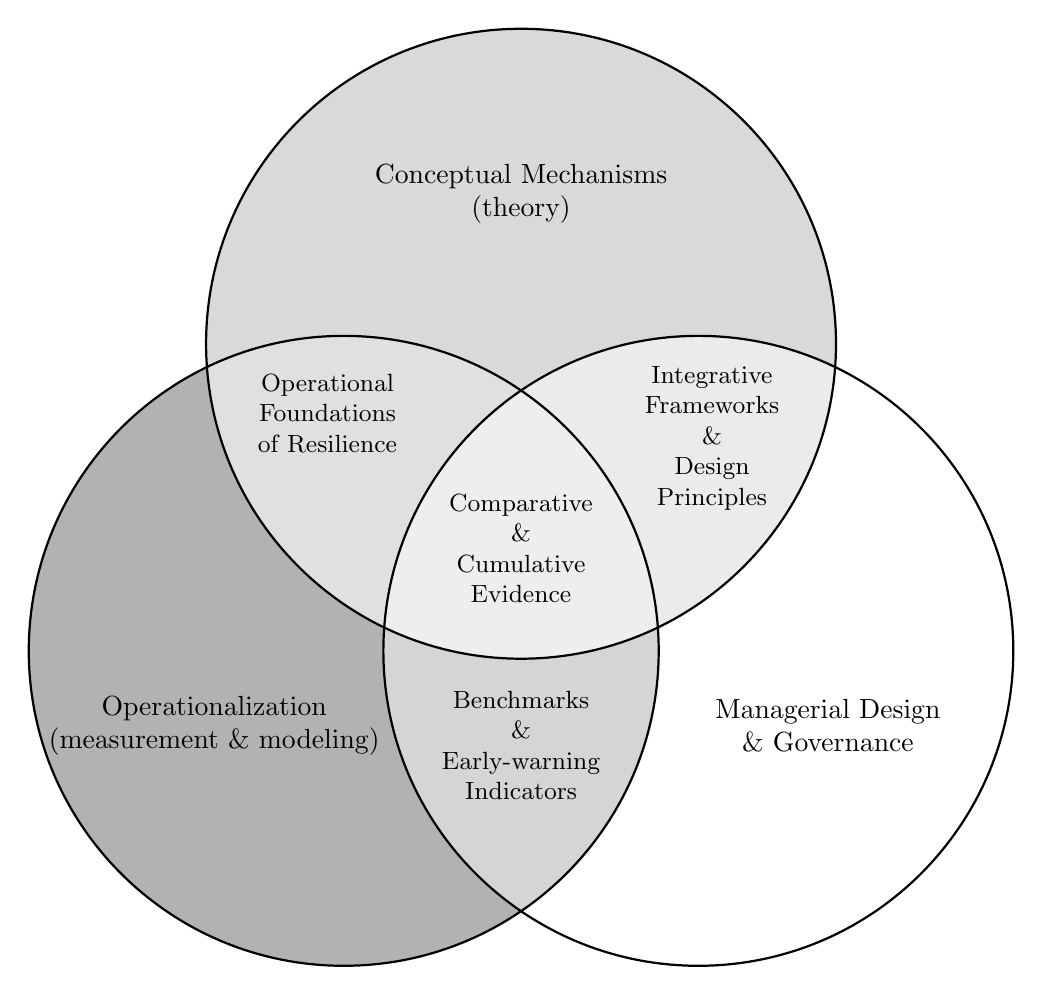
\begin{tikzpicture}
    \begin{scope}[blend group = soft light]
    \fill[gray!30!white] (90:2.6) circle (4);
    \fill[black!30!white] (210:2.6) circle (4);
    \fill[white!30!white] (330:2.6) circle (4);
    \end{scope}

    \draw[thick] (90:2.6)  circle (4);
    \draw[thick] (210:2.6) circle (4);
    \draw[thick] (330:2.6) circle (4);
    
    \node[align=center] at ( 90:4.5)    {Conceptual Mechanisms \\ (theory)};
    \node[align=center] at ( 210:4.5)   {Operationalization \\ (measurement \& modeling)};
    \node[align=center] at ( 330:4.5)   {Managerial Design \\ \& Governance};
    \node[align=center, font = \small] at ( 145:3)   {Operational\\Foundations\\ of Resilience};
    \node[align=center, font = \small] at (  30:2.8)   {Integrative\\Frameworks\\\&\\Design\\Principles};
    \node[align=center, font = \small] at ( 270:2.5)   {Benchmarks\\ \& \\Early-warning \\Indicators};
    \node[align=center, font = \small] {Comparative\\ \& \\Cumulative \\Evidence};
    \end{tikzpicture}
    \caption{From rhetoric to enactment via interfaces. The three pillars: (A) conceptual mechanisms, (B) operationalization (measurement \& modeling), and (C) managerial design \& governance -- each fails when pursued in isolation (A: rhetorical resilience; B: metrics theater; C: checkbox compliance). Resilience becomes actionable in the pairwise interfaces (A$\cap$B: operationalized mechanisms; A$\cap$C: design principles \& decision rights; B$\cap$C: benchmarks \& early-warning tied to incentives), which converge in the triple overlap (A$\cap$B$\cap$C): \emph{enacted organizational resilience}. This visual mirrors the paper’s shift from ambiguity and compliance to measurable, governed capability.}
    \label{fig:VennD}
\end{figure}






